% !TeX spellcheck = en_US
\documentclass{article}

\usepackage{listings}
\usepackage{graphicx}
\usepackage{color}

\definecolor{dkgreen}{rgb}{0,0.6,0}
\definecolor{gray}{rgb}{0.5,0.5,0.5}
\definecolor{mauve}{rgb}{0.58,0,0.82}

\lstset{frame=tb,
	language=Python,
	aboveskip=3mm,
	belowskip=3mm,
	showstringspaces=false,
	columns=flexible,
	basicstyle={\small\ttfamily},
	numbers=none,
	numberstyle=\tiny\color{gray},
	keywordstyle=\color{blue},
	commentstyle=\color{dkgreen},
	stringstyle=\color{mauve},
	breaklines=true,
	breakatwhitespace=true,
	tabsize=3
}


\usepackage{hyperref}
\hypersetup{
	colorlinks=true,
	linkcolor=blue,
	filecolor=magenta,      
	urlcolor=cyan,
	pdftitle={Overleaf Example},
	pdfpagemode=FullScreen,
}

\urlstyle{same}



\begin{document}
\title{Object Oriented Programing with Python}
\date{05/03/2024}
\author{Lucas Gonzalez Sonnenberg}
\begin{figure}
	\centering
	
\includegraphics[width=0.7\linewidth]{/home/lucas/workspace/OOP/images/logo}

\end{figure}

\maketitle
\tableofcontents
\pagebreak

\textbf{Tutorial URL}:
\url{https://www.youtube.com/watch?v=Ej_02ICOIgs&t=107s}

\section{Creating an object with a class (basic):}
\begin{lstlisting}
class Item:
	pass

item1 = 'Phone'
item1_price = 100
item1_quantity = 5
item1_price_total = item1_price * item1_quantity
\end{lstlisting}

\section{Creating the first method}
Methods are functions inside classes.

How we can go ahead and design some methods, which are going to be allowed to be executed on our instances?

The answer is, the methods should be created inside our class.

\begin{lstlisting}
class Item:
	def calculate_total_price(self):
		pass
	
	
item1 = Item()
item1_price = 100
item1_quantity = 5
item1_price_total = item1_price * item1_quantity
\end{lstlisting}

\section{Self}
Python passes the object itself as the first argument everytime. So we are not allowed to create methods without the self. 

\begin{lstlisting}
class Item:
	def calculate_total_price(self, x, y):  # x, and y are parameters
		return x * y


item1 = Item()
item1.name = "Phone"
item1.price = 100
item1.quantity = 5
print(item1.calculate_total_price(item1.price, item1.quantity))  # When I call the method calculate_total_price, Python passes the variables as mehtods.
\end{lstlisting}

\section{Magic Methods:}

\textbf{\_\_init\_\_}\\

\noindent\textbf{Instance Attributes}:\\
An instance attribute is a Python variable belonging to one, and only one, object. This variable is only accessible in the scope of this object, and it's defined inside the constructor function, \_\_init\_\_(self,..) of the class.

\begin{lstlisting}
	class Item:
		def __init__(self):  # Python executes the init function automatically.
			print("I AM CREATED")
			
		
item1 = Item()
item1_name = "Phone"
item1.price = 100
item1_quantity = 5
		
		
item1 = Item()
item_name = "Laptop"
item1_price = 1000
item1_quantity = 3


Output:
	I AM CREATED
	I AM CREATED
	
\end{lstlisting}
How to avoid creating the whole attribute, adding more parameters into the class:Assign the attributes dinamicaly. 
\begin{lstlisting}
class Item:
	def __init__(self, name):
		self.name = name
		print(f"An instance created from instance: {name}")
	
	
item1 = Item("Phone")
#item1.name = "Phone"
item1.price = 100
item1_quantity = 5
	
item2 = Item("Laptop")
#item2.name = "Laptop("
item2_price = 1000
item2.quantity = 3
	
An instance created from instance: Phone
An instance created from instance: Laptop
	
\end{lstlisting}


\begin{lstlisting}
class Item:
	def __init__(self, name):
		self.name = name
		print(f"An instance created from instance: {name}")
	
	
item1 = Item("Phone")
#item1.name = "Phone"
item1.price = 100
item1_quantity = 5
	
item2 = Item("Laptop")
#item2.name = "Laptop("
item2_price = 1000
item2.quantity = 3
	
Output:	
An instance created from instance: Phone
An instance created from instance: Laptop
	
\end{lstlisting}
\section{Simplification / Improvement of objects:}
Here is important to observe, that we can simplify the creation of objects adding the attributes to the class. Self is always mandatory.

\begin{lstlisting}
class Item:
	def __init__(self, name, price, quantity = 0):
		self.name = name
		self.price = price
		self.quantity = quantity
	
	def calculate_total_price(self):
		return self.price * self.quantity



item1 = Item("Phone", 10, 2)
item2 = Item('Laptop', 50, 15)

print(item1.calculate_total_price())
print(item2.calculate_total_price())

Output:
20
750
	 
\end{lstlisting}

\section{Delimiting data types in the class attributes.}

\begin{lstlisting}
class Item:
	def __init__(self, name: str, price: float, quantity = 0):
		#Run validations to the received arguments
		assert price >= 0
		assert quantity >= 0
		
		self.name = name
		self.price = price
		self.quantity = quantity
		
	def calculate_revenues(self):
		return self.price * self.quantity
	
	

item1 = Item("Phone", "ten", 2)
item2 = Item('Laptop', 50, 15)

print(item1.calculate_revenues())
print(item2.calculate_revenues())

Output:
Traceback (most recent call last):
File "/home/lucas/workspace/OOP/test.py", line 16, in <module>
item1 = Item("Phone", "ten", 2)
File "/home/lucas/workspace/OOP/test.py", line 4, in __init__
assert price >= 0
TypeError: '>=' not supported between instances of 'str' and 'int'
	
\end{lstlisting}

\section{Assertion Error: Technick to find quicklier the errors in the objects input}
Assert statement allows us to validate the data types of the objects and to identify errors quicklier.

\begin{lstlisting}
class Item:   
    def __init__(self, name: str, price: float, quantity = 0):
		#Run validations to the received arguments
		assert price >= 0, f"Price is lower than 0"
		assert quantity >= 0, f"Quantity is lower than 0"
		
		self.name = name
		self.price = price
		self.quantity = quantity
	
	def calculate_revenues(self):
		return self.price * self.quantity
	


item1 = Item("Phone", 2, -2)
item2 = Item('Laptop', 50, 15)

print(item1.calculate_revenues())
print(item2.calculate_revenues())

Output:

/usr/bin/python3.10 /home/lucas/workspace/OOP/test.py 
Traceback (most recent call last):
File "/home/lucas/workspace/OOP/test.py", line 16, in <module>
item1 = Item("Phone", 2, -2)
File "/home/lucas/workspace/OOP/test.py", line 5, in __init__
assert quantity >= 0, f"Quantity is lower than 0"
AssertionError: Quantity is lower than 0

Process finished with exit code 1
\end{lstlisting}

\section{Class Attributes}
Class attributes are like global attributes. They belong to the class, but they can also be reached from the instance aswell. 

For this example I used pay\_rate as a class attribute.

\begin{lstlisting}
class Item:
	pay_rate = 0.8
	def __init__(self, name: str, price: float, quantity = 0):
		#Run validations to the received arguments
		assert price >= 0, f"Price is lower than 0"
		assert quantity >= 0, f"Quantity is lower than 0"
	
		#Instance Level
		self.name = name
		self.price = price
		self.quantity = quantity
		
	def calculate_revenues(self):
		return self.price * self.quantity
	


item1 = Item("Phone", 2, 2)
item2 = Item('Laptop', 50, 15)

print(item1.pay_rate)
print(item2.pay_rate)

Output:
/usr/bin/python3.10 /home/lucas/workspace/OOP/test.py 
0.8
0.8

Process finished with exit code 0
	
\end{lstlisting}

\section{Magic Attriute:}
To see all the existent attributes: \_\_dict\_\_
This is used to see all the attributes belonging to an object.

\begin{lstlisting}
class Item:
	#Class Level
	pay_rate = 0.8
	def __init__(self, name: str, price: float, quantity = 0):
		#Run validations to the received arguments
		assert price >= 0, f"Price is lower than 0"
		assert quantity >= 0, f"Quantity is lower than 0"
	
		#Instance Level
		self.name = name
		self.price = price
		self.quantity = quantity
		
	def calculate_revenues(self):
		return self.price * self.quantity
	
	

item1 = Item("Phone", 2, 2)
item2 = Item('Laptop', 50, 15)

print(f"These are all the class level attributes: {Item.__dict__}")
print(f"These are all the instance level attributes: {item1.__dict__}")

Output:
/usr/bin/python3.10 /home/lucas/workspace/OOP/test.py 
These are all the class level attributes: {'__module__': '__main__', 'pay_rate': 0.8, '__init__': <function Item.__init__ at 0x7ff8de22a0e0>, 'calculate_revenues': <function Item.calculate_revenues at 0x7ff8de22a440>, '__dict__': <attribute '__dict__' of 'Item' objects>, '__weakref__': <attribute '__weakref__' of 'Item' objects>, '__doc__': None}
These are all the instance level attributes: {'name': 'Phone', 'price': 2, 'quantity': 2}

Process finished with exit code 0
\end{lstlisting}

\section{Accessing a class attribute from a method}

\begin{lstlisting}
class Item:
	#Class Level
	pay_rate = 0.8
	def __init__(self, name: str, price: float, quantity = 0):
		#Run validations to the received arguments
		assert price >= 0, f"Price is lower than 0"
		assert quantity >= 0, f"Quantity is lower than 0"
		
		#Instance Level
		self.name = name
		self.price = price
		self.quantity = quantity
	
	def calculate_revenues(self):
		return self.price * self.quantity
	
	def apply_discount(self):
		self.price = self.price * Item.pay_rate



item1 = Item("Phone", 15000, 2)
item1.apply_discount()
print(item1.price)

Output:
/usr/bin/python3.10 /home/lucas/workspace/OOP/test.py 
12000.0

Process finished with exit code 0


\end{lstlisting}

\section{Modify a class attribute for an specific instance}:

\begin{lstlisting}
class Item:
	#Class Level
	pay_rate = 0.8
	def __init__(self, name: str, price: float, quantity = 0):
		#Run validations to the received arguments
		assert price >= 0, f"Price is lower than 0"
		assert quantity >= 0, f"Quantity is lower than 0"
		
		#Instance Level
		self.name = name
		self.price = price
		self.quantity = quantity
		
	def calculate_revenues(self):
		return self.price * self.quantity
		
	def apply_discount(self):
		self.price = self.price * self.pay_rate # It is important to change Item with self. If not, the pay rate will not be read from the instance, rather from the class. Without this modification, it will be changed on the instance.
		
	
	
item1 = Item("Phone", 100, 2)
item1.apply_discount()
print(f'The price of {item1.name} is {item1.price}')
	
item2 = Item("Laptop", 1500, 1)
item2.pay_rate = 0.9
item2.apply_discount()
print(f'The price of {item2.name} is {item2.price}')

Output:
/usr/bin/python3.10 /home/lucas/workspace/OOP/test.py 
The price of Phone is 80.0
The price of Laptop is 1350.0

Process finished with exit code 0

\end{lstlisting}

\section{Working with multiple instances:}
We create a list, and we append all items from Item to the list all.

\begin{lstlisting}
	class Item:
		#Class Level
		pay_rate = 0.8
		all = []
		def __init__(self, name: str, price: float, quantity = 0):
			#Run validations to the received arguments
			assert price >= 0, f"Price is lower than 0"
			assert quantity >= 0, f"Quantity is lower than 0"
			
			#Assign to self object
			self.name = name
			self.price = price
			self.quantity = quantity
			
			#Actions to execute
			Item.all.append(self)
			
		def calculate_revenues(self):
			return self.price * self.quantity
		
		def apply_discount(self):
			self.price = self.price * self.pay_rate
		
		
		
item1 = Item("Phone", 100, 1)
item2 = Item("Laptop", 1000, 3)
item3 = Item("Cable", 10, 5)
item4 = Item("Mouse", 50, 5)
item5 = Item("Keyboard", 75, 5)
		
for instance in Item.all:
	print(instance.name)	

Output:
/usr/bin/python3.10 /home/lucas/workspace/OOP/test.py 
Phone
Laptop
Cable
Mouse
Keyboard

Process finished with exit code 0	
	
\end{lstlisting}

\section{Magic Method: \_\_repr\_\_}
repr: means representing your objects
It's a good tool to handle the different objects.
\begin{lstlisting}
	class Item:
		#Class Level
		pay_rate = 0.8
		all = []
		def __init__(self, name: str, price: float, quantity = 0):
			#Run validations to the received arguments
			assert price >= 0, f"Price is lower than 0"
			assert quantity >= 0, f"Quantity is lower than 0"
			
			#Assign to self object
			self.name = name
			self.price = price
			self.quantity = quantity
			
			#Actions to execute
			Item.all.append(self)
			
		def calculate_revenues(self):
			return self.price * self.quantity
			
		def apply_discount(self):
			self.price = self.price * self.pay_rate
			
		def __repr__(self):
			return f"Item name:{self.name}, price: {self.price}, and quantity: {self.quantity}"
			
	
	
	item1 = Item("Phone", 100, 1)
	item2 = Item("Laptop", 1000, 3)
	item3 = Item("Cable", 10, 5)
	item4 = Item("Mouse", 50, 5)
	item5 = Item("Keyboard", 75, 5)
	
	
	
	print(Item.all)
	
Output:
/usr/bin/python3.10 /home/lucas/workspace/OOP/test.py 
[Item name:Phone, price: 100, and quantity: 1, Item name:Laptop, price: 1000, and quantity: 3, Item name:Cable, price: 10, and quantity: 5, Item name:Mouse, price: 50, and quantity: 5, Item name:Keyboard, price: 75, and quantity: 5]

Process finished with exit code 0
\end{lstlisting}

The \_\_repr\_\_ magic method is also useful to show the objects in a form directly usable to transfer them to another python user. This is part of the best practices according to python document.

\begin{lstlisting}
	class Item:
		#Class Level
		pay_rate = 0.8
		all = []
		def __init__(self, name: str, price: float, quantity = 0):
			#Run validations to the received arguments
			assert price >= 0, f"Price is lower than 0"
			assert quantity >= 0, f"Quantity is lower than 0"
			
			#Assign to self object
			self.name = name
			self.price = price
			self.quantity = quantity
			
			#Actions to execute
			Item.all.append(self)
			
		def calculate_revenues(self):
			return self.price * self.quantity
		
		def apply_discount(self):
			self.price = self.price * self.pay_rate
		
		def __repr__(self):
			return f"Item({self.name}, {self.price}, {self.quantity})"
		
		
		
	
	item1 = Item("Phone", 100, 1)
	item2 = Item("Laptop", 1000, 3)
	item3 = Item("Cable", 10, 5)
	item4 = Item("Mouse", 50, 5)
	item5 = Item("Keyboard", 75, 5)
	
	
	
	print(Item.all)
	
Output:
/usr/bin/python3.10 /home/lucas/workspace/OOP/test.py 
[Item(Phone, 100, 1), Item(Laptop, 1000, 3), Item(Cable, 10, 5), Item(Mouse, 50, 5), Item(Keyboard, 75, 5)] #We recibe a list, which is more friendly.
The first element is equal to the first object, and so on.
	
	Process finished with exit code 0
\end{lstlisting}

\section{Class Method}
Definition:\\
A class method is a method that is bound to the class and not the object of the class. They have the access to the state of the class as it takes a class parameter that points to the class and not the object instance. It can modify a class state that would apply across all the instances of the class.\\


For this I created a csv file named "csv.csv". The content of the file is as follows:\\


\noindent name, price, quantity\\
\noindent"Phone", 100, 1\\
\noindent"Laptop", 1000, 3\\
\noindent"Cable", 10, 5\\
\noindent"Mouse", 50, 5\\
\noindent"Keyboard", 75, 5\\

\begin{lstlisting}
	import csv
	
	class Item:
		#Class Level
		pay_rate = 0.8
		all = []
		def __init__(self, name: str, price: float, quantity = 0):
		#Run validations to the received arguments
		assert price >= 0, f"Price is lower than 0"
		assert quantity >= 0, f"Quantity is lower than 0"
		
		#Assign to self object
		self.name = name
		self.price = price
		self.quantity = quantity
		
		#Actions to execute
		Item.all.append(self)
		
		def calculate_revenues(self):
			return self.price * self.quantity
		
		def apply_discount(self):
			self.price = self.price * self.pay_rate
		
		@classmethod
		def instantiate_from_csv(cls):
			with open('csv.csv', 'r') as f:
			reader = csv.DictReader(f)
			items = list(reader)
			
			for item in items:
			print(item)
			
		def __repr__(self):
			return f"Item({self.name}, {self.price}, {self.quantity})"
			
	
	Item.instantiate_from_csv()
	
Output:
/usr/bin/python3.10 /home/lucas/workspace/OOP/test.py 
{'name': 'Phone', ' price': ' 100', ' quantity': ' 1'}
{'name': 'Laptop', ' price': ' 1000', ' quantity': ' 3'}
{'name': 'Cable', ' price': ' 10', ' quantity': ' 5'}
{'name': 'Mouse', ' price': ' 50', ' quantity': ' 5'}
{'name': 'Keyboard', ' price': ' 75', ' quantity': ' 5'}

Process finished with exit code 0
	
\end{lstlisting}

\section{Creating instances using the class method:}

\begin{lstlisting}
	
	import csv
	
	class Item:
		#Class Level
		pay_rate = 0.8
		all = []
		def __init__(self, name: str, price: float, quantity = 0):
			#Run validations to the received arguments
			assert price >= 0, f"Price is lower than 0"
			assert quantity >= 0, f"Quantity is lower than 0"
			
			#Assign to self object
			self.name = name
			self.price = price
			self.quantity = quantity
			
			#Actions to execute
			Item.all.append(self)
			
		def calculate_revenues(self):
			return self.price * self.quantity
			
		def apply_discount(self):
			self.price = self.price * self.pay_rate
		
		@classmethod
		def instantiate_from_csv(cls):
			with open('csv.csv', 'r') as f:
			reader = csv.DictReader(f)
			items = list(reader)
			
			for item in items:
			Item(
			name = item.get('name'),
			price = float(item.get('price')),
			quantity = int(item.get('quantity'))
			)
			
		def __repr__(self):
			return f"Item({self.name}, {self.price}, {self.quantity})"
		
		
	Item.instantiate_from_csv()
	print(Item.all)
	
Output:
/usr/bin/python3.10 /home/lucas/workspace/OOP/test.py 
[Item(Phone, 100.0, 1), Item(Laptop, 1000.0, 3), Item(Cable, 10.0, 5), Item(Mouse, 50.0, 5), Item(Keyboard, 74.5, 5)]

Process finished with exit code 0
\end{lstlisting}

\section{Static Method}
The static method never sends the object as the first argument.

\begin{lstlisting}
	
	import csv
	
	class Item:
		#Class Level
		pay_rate = 0.8
		all = []
		def __init__(self, name: str, price: float, quantity = 0):
			#Run validations to the received arguments
			assert price >= 0, f"Price is lower than 0"
			assert quantity >= 0, f"Quantity is lower than 0"
			
			#Assign to self object
			self.name = name
			self.price = price
			self.quantity = quantity
			
			#Actions to execute
			Item.all.append(self)
		
		def calculate_revenues(self):
			return self.price * self.quantity
			
		def apply_discount(self):
			self.price = self.price * self.pay_rate
			
		@classmethod
		def instantiate_from_csv(cls):
			with open('csv.csv', 'r') as f:
				reader = csv.DictReader(f)
				items = list(reader)
			
			for item in items:
				Item(
				name = item.get('name'),
				price = float(item.get('price')),
				quantity = int(item.get('quantity'))
				)

		@staticmethod
		def is_integer(num):
			#We will count out the floats that are point zero.
			#For i.e.: 5.0, 10.0
			if isinstance(num, float):
			#Count out the floats that are point zero
			return num.is_integer()
			elif isinstance(num, int):
			return True
			else:
			return False
			
		def __repr__(self):
			return f"Item({self.name}, {self.price}, {self.quantity})"
			
		
	
	print(Item.is_integer(7.5))
	print(Item.is_integer(8.0))
	
	Output:
	/usr/bin/python3.10 /home/lucas/workspace/OOP/test.py 
	False
	True
	
	Process finished with exit code 0
	
\end{lstlisting}

\section{static Method vs class Method}
\textbf{static method}: It is used to do something that has a relationship with the class, but not something that must be unique per instance.

Static method are not passing the object reference as the first argument in the background. They use a \textbf{regular} parameter, which is not mandatory.

\begin{lstlisting}
	class Item:
		@staticmethod:
		def is_integer():
\end{lstlisting}

\textbf{class method}: It is used to do something that has a relationship with the class, but usually, those that are used to manipulate different structures of data to instantiate objects, like we have done with CSV.

Class method are passing the object reference as the first argument in the background. They use a \textbf{mandatory} parameter, which is not mandatory.

\begin{lstlisting}
	class Item:
		@classmethod:
		def instantiate_from_something(cls):
\end{lstlisting}

\section{Inheritance}

It is used to give extra functionalities to the instances, which are special.
These instances have something, which make them special. For example a company, which sells phones. These company have 2 broken phones. They havo to give them the category of broken, but this category is required only for 2 phones.

In order to solve this problem I have to create a new category, with all the aspects of the old one. Then I have to add these special features to the new category. 

For this example, I'm using the inheritance. I created a new class called Phone, which departs from the first class named Item. I'm not adding any special feature to the class Phone yet. But we can observe, that there is not error using the class Phone instead of Item.

\begin{lstlisting}
	import csv
	
	class Item:
		#Class Level
		pay_rate = 0.8
		all = []
		def __init__(self, name: str, price: float, quantity = 0):
			#Run validations to the received arguments
			assert price >= 0, f"Price is lower than 0"
			assert quantity >= 0, f"Quantity is lower than 0"
			
			#Assign to self object
			self.name = name
			self.price = price
			self.quantity = quantity
			
			#Actions to execute
			Item.all.append(self)
			
		def calculate_revenues(self):
			return self.price * self.quantity
			
		def apply_discount(self):
			self.price = self.price * self.pay_rate
			
			@classmethod
		def instantiate_from_csv(cls):
			with open('csv.csv', 'r') as f:
			reader = csv.DictReader(f)
			items = list(reader)
			
			for item in items:
			Item(
			name = item.get('name'),
			price = float(item.get('price')),
			quantity = int(item.get('quantity'))
			)
		@staticmethod
		def is_integer(num):
			#We will count out the floats that are point zero.
			#For i.e.: 5.0, 10.0
			if isinstance(num, float):
			#Count out the floats that are point zero
			return num.is_integer()
			elif isinstance(num, int):
			return True
			else:
			return False
		
		def __repr__(self):
			return f"Item({self.name}, {self.price}, {self.quantity})"
	
	class Phone(Item):
		pass
	
	
	phone1 = Phone("jscPhonev10", 500, 5)
	phone2 = Phone("jscPhonev20", 700, 5)
	
Output: 
/usr/bin/python3.10 /home/lucas/workspace/OOP/test.py 

Process finished with exit code 0


\end{lstlisting}

\section{Parent Classes}
These related classes are composed by parent classes and a child classes. 


\begin{figure}[ht]
	\centering
	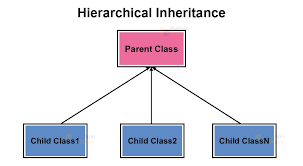
\includegraphics[width=0.7\linewidth]{/home/lucas/workspace/OOP/images/images}
	\caption{}
	\label{fig:images}
\end{figure}

\section{Super}
Super allows us to have full access to all the attributes of the parent class. By using the \textbf{super} function we don't need to copy the old class. It is enough, if we add the new attributes.

\begin{lstlisting}
	import csv
	
	class Item:
		#Class Level
		pay_rate = 0.8
		all = []
		def __init__(self, name: str, price: float, quantity = 0):
			#Run validations to the received arguments
			assert price >= 0, f"Price is lower than 0"
			assert quantity >= 0, f"Quantity is lower than 0"
			
			#Assign to self object
			self.name = name
			self.price = price
			self.quantity = quantity
			
			#Actions to execute
			Item.all.append(self)
			
		def calculate_revenues(self):
			return self.price * self.quantity
		
		def apply_discount(self):
			self.price = self.price * self.pay_rate
			
		@classmethod
		def instantiate_from_csv(cls):
			with open('csv.csv', 'r') as f:
				reader = csv.DictReader(f)
				items = list(reader)
			
			for item in items:
				Item(
					name = item.get('name'),
					price = float(item.get('price')),
					quantity = int(item.get('quantity'))
				)
		@staticmethod
		def is_integer(num):
			#We will count out the floats that are point zero.
			#For i.e.: 5.0, 10.0
			if isinstance(num, float):
			#Count out the floats that are point zero
				return num.is_integer()
			elif isinstance(num, int):
				return True
			else:
				return False
			
		def __repr__(self):
			return f"Item({self.name}, {self.price}, {self.quantity})"
	
	class Phone(Item):
		all = []
		def __init__(self, name, price, quantity, broken_phones = 0):
			#Call to super function to have acces to all attributes and methods
			super().__init__(
			name, price, quantity
			)
			#Run validations to received arguments
			assert broken_phones >= 0, f"Broken Phones {broken_phones} is not greater or equal than 0"
			
			#Actions to execute
			Phone.all.append(self)
			
	
	phone1 = Phone("jscPhonev10", 500, 5)
	print(phone1.calculate_revenues())
	phone2 = Phone("jscPhonev20", 700, 5)
	
Output:
/usr/bin/python3.10 /home/lucas/workspace/OOP/test.py 
[Item(jscPhonev10, 500, 5), Item(jscPhonev20, 700, 5)] 
[Item(jscPhonev10, 500, 5), Item(jscPhonev20, 700, 5)]
#It is not good to observe that, the broken phones still come from the class item.


Process finished with exit code 0
	
\end{lstlisting} 

\section{Separating the objects from each class}
To avoid the last error of receiving allways that the object comes from the parent class, we modified the string Item with the magic methods: \_\_class\_\_.\_\_name\_\_

\begin{lstlisting}
	def __repr__(self):
	return f"{self.__class__.__name__}({self.name}, {self.price}, {self.quantity})"
	#return f"Item(self.name}, {self.price}, {self.quantity})" we replaced this command to avoid getting allways the name of the class Item.
\end{lstlisting}

The whole code is as following:

\begin{lstlisting}
import csv


class Item:
	# Class Level
	pay_rate = 0.8
	all = []
	
def __init__(self, name: str, price: float, quantity=0):
	# Run validations to the received arguments
	assert price >= 0, f"Price is lower than 0"
	assert quantity >= 0, f"Quantity is lower than 0"
	
	# Assign to self object
	self.name = name
	self.price = price
	self.quantity = quantity
	
	# Actions to execute
	Item.all.append(self)
	
def calculate_revenues(self):
	return self.price * self.quantity

def apply_discount(self):
	self.price = self.price * self.pay_rate

@classmethod
def instantiate_from_csv(cls):
	with open('csv.csv', 'r') as f:
		reader = csv.DictReader(f)
		items = list(reader)
	
	for item in items:
		Item(
			name=item.get('name'),
			price=float(item.get('price')),
			quantity=int(item.get('quantity'))
		)
	
@staticmethod
def is_integer(num):
	# We will count out the floats that are point zero.
	# For i.e.: 5.0, 10.0
	if isinstance(num, float):
		# Count out the floats that are point zero
		return num.is_integer()
	elif isinstance(num, int):
		return True
	else:
		return False
	
def __repr__(self):
	return f"{self.__class__.__name__}({self.name}, {self.price}, {self.quantity})"
	#return f"Item(self.name}, {self.price}, {self.quantity})" we replaced this command to avoid getting allways the name of the class Item.

class Phone(Item):
	all = []
	
	def __init__(self, name, price, quantity, broken_phones=0):
		# Call to super function to have acces to all attributes and methods
		super().__init__(
		name, price, quantity
		)
		# Run validations to received arguments
		assert broken_phones >= 0, f"Broken Phones {broken_phones} is not greater or equal than 0"
		
		#Actions to execute
		Phone.all.append(self)


phone1 = Phone("jscPhonev10", 500, 5)
phone2 = Phone("jscPhonev20", 700, 5)
print(Item.all)
print(Phone.all)

Output:
/usr/bin/python3.10 /home/lucas/workspace/OOP/test.py 
[Phone(jscPhonev10, 500, 5), Phone(jscPhonev20, 700, 5)] 
[Phone(jscPhonev10, 500, 5), Phone(jscPhonev20, 700, 5)] 
#Now we can observe the change.
Process finished with exit code 0

\end{lstlisting}
\section{More uses of the super function}
It is a good idea to remove all the imported methods and attributes from the parent class. In this case we removed the append function and the "all" attribute. The output is still the same result.

\section{Getters and Setters}
The project is growing, so we need to start working with multiple files.
A good idea is to have a file that represents the Parent Class, and another file, which represents the Child Class.

So now we have 3 files:
\begin{itemize}
	\item main
	\item item
	\item phone
\end{itemize}

\textbf{item:}
\begin{lstlisting}
import csv


class Item:
	# Class Level
	pay_rate = 0.8
	all = []
	
	def __init__(self, name: str, price: float, quantity=0):
		# Run validations to the received arguments
		assert price >= 0, f"Price is lower than 0"
		assert quantity >= 0, f"Quantity is lower than 0"
		
		# Assign to self object
		self.name = name
		self.price = price
		self.quantity = quantity
		
		# Actions to execute
		Item.all.append(self)
		
	def calculate_revenues(self):
		return self.price * self.quantity
		
	def apply_discount(self):
		self.price = self.price * self.pay_rate
		
	@classmethod
	def instantiate_from_csv(cls):
		with open('instances.csv', 'r') as f:
			reader = csv.DictReader(f)
			items = list(reader)
		
		for item in items:
			Item(
				name=item.get('name'),
				price=float(item.get('price')),
				quantity=int(item.get('quantity'))
			)
		
	@staticmethod
	def is_integer(num):
		# We will count out the floats that are point zero.
		# For i.e.: 5.0, 10.0
		if isinstance(num, float):
			# Count out the floats that are point zero
			return num.is_integer()
		elif isinstance(num, int):
			return True
		else:
			return False
	
	def __repr__(self):
		return f"{self.__class__.__name__}({self.name}, {self.price}, {self.quantity})"
\end{lstlisting}

\textbf{phone:}

\begin{lstlisting}
	from item import Item
	
	class Phone(Item):
		
		def __init__(self, name, price, quantity, broken_phones=0):
			# Call to super function to have acces to all attributes and methods
			super().__init__(
			name, price, quantity
			)
			# Run validations to received arguments
			assert broken_phones >= 0, f"Broken Phones {broken_phones} is not greater or equal than 0"
\end{lstlisting}

\textbf{main:}
\begin{lstlisting}
	from item import Item
	from phone import Phone
	
	phone1 = Phone("jscPhonev10", 500, 5)
	phone2 = Phone("jscPhonev20", 700, 5)
	print(Item.all)
	print(Phone.all)
\end{lstlisting}

\textbf{Output from main:}

\begin{lstlisting}
	/usr/bin/python3.10 /home/lucas/workspace/OOP/main.py 
	[Phone(jscPhonev10, 500, 5), Phone(jscPhonev20, 700, 5)]
	[Phone(jscPhonev10, 500, 5), Phone(jscPhonev20, 700, 5)]
	
	Process finished with exit code 0
\end{lstlisting}

\section{Encapsulation}

Encapsulation in Python is the concept of bundling the data (attributes) and methods (functions) that operate on the data into a single unit, called a class. It is one of the fundamental principles of object-oriented programming (OOP) and facilitates the creation of modular and reusable code.

\textbf{Encapsulation helps to hide the internal state of an object from the outside world and restricts direct access to the data}, enforcing access through well-defined methods. This allows for better control over how data is manipulated and prevents unintended modifications that could lead to errors or inconsistencies.

\noindent\textbf{Access Control:}\\
Encapsulation allows you to control the access to the attributes and methods of a class. By using access modifiers such as public, private, and protected, you can specify which parts of the class are accessible from outside the class.\\
\noindent\textbf{Data Hiding:}\\
ncapsulation hides the internal state of an object from external code. This means that the implementation details of the class are hidden and can only be accessed and modified through the defined methods.\\
\noindent\textbf{Abstraction:}\\
Encapsulation helps to achieve abstraction by exposing only the essential features of an object while hiding the complex implementation details. This allows users of the class to interact with it at a higher level of abstraction without needing to understand its internal workings.\\

\noindent\textbf{Read only attributes:}

\textbf{Item}
\begin{lstlisting}
	
	@property
	def read_only_name(self):
		return "AAA"
	
\end{lstlisting}

\textbf{main}
\begin{lstlisting}

from item import Item
from phone import Phone

item1 = Item("MyItem", 750)

item1.name = "OtherItem"

print(item1.name)
print(item1.read_only_name)

item1.read_only_name = 'BBB'

Output
/usr/bin/python3.10 /home/lucas/workspace/OOP/main.py 
OtherItem
AAA
Traceback (most recent call last):
File "/home/lucas/workspace/OOP/main.py", line 11, in <module>
item1.read_only_name = 'BBB'
AttributeError: can't set attribute 'read_only_name'

Process finished with exit code 1

	
\end{lstlisting}
\section{Setter}
After using the decorator \textbf{property}, there is a possibility to still modifying the items.
For this I have to use the decorator \textbf{setter}:

\textbf{item}

\begin{lstlisting}
import csv


class Item:
	# Class Level
	pay_rate = 0.8
	all = []
	
	def __init__(self, name: str, price: float, quantity=0):
		# Run validations to the received arguments
		assert price >= 0, f"Price is lower than 0"
		assert quantity >= 0, f"Quantity is lower than 0"
		
		# Assign to self object
		self.__name = name #name has __ to avoid accesing this variable from outside.
		self.price = price
		self.quantity = quantity
		
		# Actions to execute
		Item.all.append(self)
	
	def calculate_revenues(self):
		return self.price * self.quantity
	
	def apply_discount(self):
		self.price = self.price * self.pay_rate
	
	@classmethod
	def instantiate_from_csv(cls):
		with open('instances.csv', 'r') as f:
			reader = csv.DictReader(f)
			items = list(reader)
		
		for item in items:
			Item(
				name=item.get('name'),
				price=float(item.get('price')),
				quantity=int(item.get('quantity'))
				)
		
	@staticmethod
		def is_integer(num):
		# We will count out the floats that are point zero.
		# For i.e.: 5.0, 10.0
		if isinstance(num, float):
			# Count out the floats that are point zero
			return num.is_integer()
		elif isinstance(num, int):
			return True
		else:
			return False
	
	def __repr__(self):
		return f"{self.__class__.__name__}({self.name}, {self.price}, {self.quantity})"
	
	@property
	# Property decorator = Read-only attributes
	def name(self):
		print("You're traying to get name (decorator property)")
		return self.__name
	
	@name.setter
	#Decorator to modify variables
	def name(self, value):
		print("You're traying to get name (decorator setter)")
		self.__name = value

\end{lstlisting}

\textbf{main}

\begin{lstlisting}
from item import Item
from phone import Phone

item1 = Item("MyItem", 750)

item1.name = "OtherItem"

print(item1.name)

Output:
/usr/bin/python3.10 /home/lucas/workspace/OOP/main.py 
OtherItem

Process finished with exit code 0

\end{lstlisting}

\section{setters: Including restrictions and limitations}

With setters is also possible to delimit the new achievable values for a variable.
For example we can restrict the length of the characters of the name of an attribute.

\textbf{private attribute:} It is important to mention that, when a variable has double underscore, this is a private variable and it can't be accessed from outside the class.\\


\textbf{item:}
\begin{lstlisting}
import csv

class Item:
	# Class Level
	pay_rate = 0.8
	all = []
	
	def __init__(self, name: str, price: float, quantity=0):
		# Run validations to the received arguments
		assert price >= 0, f"Price is lower than 0"
		assert quantity >= 0, f"Quantity is lower than 0"
		
		# Assign to self object
		self.__name = name
		self.price = price
		self.quantity = quantity
		
		# Actions to execute
		Item.all.append(self)
		
	def calculate_revenues(self):
		return self.price * self.quantity
		
	def apply_discount(self):
		self.price = self.price * self.pay_rate
		
	@classmethod
	def instantiate_from_csv(cls):
		with open('instances.csv', 'r') as f:
			reader = csv.DictReader(f)
			items = list(reader)
			
		for item in items:
			Item(
			name=item.get('name'),
			price=float(item.get('price')),
			quantity=int(item.get('quantity'))
			)
		
	@staticmethod
	def is_integer(num):
		# We will count out the floats that are point zero.
		# For i.e.: 5.0, 10.0
		if isinstance(num, float):
			# Count out the floats that are point zero
			return num.is_integer()
		elif isinstance(num, int):
			return True
		else:
			return False
	
	def __repr__(self):
		return f"{self.__class__.__name__}({self.name}, {self.price}, {self.quantity})"
	
	@property
	# Property decorator = Read-only attributes
	def name(self):
		print("You're getting name from decorator property)")
		return self.__name
		
	@name.setter
	#Decorator to modify variables
	def name(self, value):
		if len(value) > 10:
			raise Exception(f"Name: {value} is too long.") #Here it is nice to see how to create an exception.
		else:
			self.__name = value
			print(f'New name {value} accepted')
\end{lstlisting}

\textbf{main}
\begin{lstlisting}
	from item import Item
	from phone import Phone
	
	item1 = Item("MyItem", 750)
	
	item1.name = "Brkn_item"
	
	print(item1.name)
\end{lstlisting}

\textbf{Output}

\begin{lstlisting}
	/usr/bin/python3.10 /home/lucas/workspace/OOP/main.py 
	New name Brkn_item accepted
	You're getting name from decorator property)
	Brkn_item
	
	Process finished with exit code 0
\end{lstlisting}

\section{OOB}
\begin{itemize}
	\item \textbf{Encapsulation:}\\
	It describes the idea of wrapping (envolver) data and the methods that work on data within one unit. This puts \textbf{restrictions on accessing variables and methods} directly and can prevent the accidental modification of data.
	
	\item \textbf{Abstraction:}\\
	It refers to the concept of \textbf{hiding the complex implementation} details of a piece of code while \textbf{providing a simple and clear interface} for interacting with it. 
	Only show the necessary attributes, and hide the unnecessary.
	To achieve this is possible to create the methods from the class method, and then hiding them with \_\_.\\
	
	\item \textbf{Inheritance}\\
	This concept allows a class (known as the child or derived class) to inherit attributes and methods from another class (known as the parent or base class). This enables us to reuse codes and promotes a hierarchical organization of classes.\\
	\item \textbf{Polymorphism}\\
	allows objects of different classes to be treated as objects of a common superclass. This enables a single interface to be used for entities of different types, promoting flexibility and code reusability.\\
\end{itemize}


\section{Encapsulation}
Firstly, we change the price attribute to be a private attribute adding \_\_.
Secondly, we create a \textbf{property decorator} to make, that this variable is just a read variable. At this point we can't modify the variable price anymore.
Thirdly, we create two new decorators, one to increase the price of the instance named: \textbf{apply\_increment}, and a second one called \textbf{apply\_discount}.

\textbf{item:}
\begin{lstlisting}
	import csv
	
	class Item:
		# Class Level
		pay_rate = 0.8
		all = []
		
		def __init__(self, name: str, price: float, quantity=0):
			# Run validations to the received arguments
			assert price >= 0, f"Price is lower than 0"
			assert quantity >= 0, f"Quantity is lower than 0"
			
			# Assign to self object
			self.__name = name
			self.__price = price
			self.quantity = quantity
			
			# Actions to execute
			Item.all.append(self)
		
		def calculate_revenues(self):
			return self.__price * self.quantity
			
		@classmethod
		def instantiate_from_csv(cls):
			with open('instances.csv', 'r') as f:
				reader = csv.DictReader(f)
				items = list(reader)
			
			for item in items:
				Item(
				name=item.get('name'),
				price=float(item.get('price')),
				quantity=int(item.get('quantity'))
				)
				
		@staticmethod
		def is_integer(num):
			# We will count out the floats that are point zero.
			# For i.e.: 5.0, 10.0
			if isinstance(num, float):
				# Count out the floats that are point zero
				return num.is_integer()
			elif isinstance(num, int):
				return True
			else:
				return False
			
		def __repr__(self):
			return f"{self.__class__.__name__}({self.name}, {self.__price}, {self.quantity})"
		
		@property
		#Property decorator = Read-only attribute
		def price(self):
			return self.__price
		
		def apply_discount(self):
			self.__price = self.__price * self.pay_rate
		
		def apply_increment(self, increment_value):
			self.__price = self.__price + self.__price * increment_value
		
		@property
		# Property decorator = Read-only attributes
		def name(self):
			print("You're getting name from decorator property)")
			return self.__name
		
		
		@name.setter
		#Decorator to modify variables
		def name(self, value):
			if len(value) > 10:
				raise Exception(f"Name: {value} is too long.")
			else:
				self.__name = value
				print(f'New name {value} accepted')
\end{lstlisting}

\textbf{main}

\begin{lstlisting}
from item import Item
from phone import Phone

item1 = Item("MyItem", 750)
item1.apply_discount()

print(f'Product: {item1.name}, price: {item1.price}')
item2 = Item('Second_item', 600)
item2.apply_increment(0.25)
print(f'Product: {item2.name}, price: {item2.price}')

Output:
/usr/bin/python3.10 /home/lucas/workspace/OOP/main.py 
Product: MyItem, price: 600.0
Product: Second_item, price: 750.0

Process finished with exit code 0	
\end{lstlisting}

\textbf{Polymorphism}\\
A good example of this OOB attribute is the len function. 
If we use the len function on a string, we get back the number of letters in that string.
But if we use the len function on a list, we get the number of elements belonging to that list.

It is a single entity, that knows how to handle different kinds of objects.

\begin{lstlisting}
	name = 'Lucas'
	list = ['bananas', 'tomatoes']
	
	print(f'Count the number of letters in a string: {len(list)}')
	print(f'Count the number of elements in a list: {len(list)}')
	
	Output:
	
	/usr/bin/python3.10 /home/lucas/workspace/OOP/Polymorphism.py 
	Count the number of letters in a string: 2
	Count the number of elements in a list: 2
	
	Process finished with exit code 0
\end{lstlisting}
Another example of polymorphism is the apply\_discount function created on the class Item, which we are using in the new class keyboard, without defining it again. 

\textbf{keyboard}
\begin{lstlisting}
	from item import Item
	
	class Keyboard(Item):
		pay_rate = 0.89
		def __init__(self, name, price, quantity, broken_phones=0):
			# Call to super function to have acces to all attributes and methods
			super().__init__(
			name, price, quantity
			)
	
\end{lstlisting}

\textbf{main}
\begin{lstlisting}
	from item import Item
	from keyboard import Keyboard
	
	item1 = Keyboard('keyboard_1', 175, 3)
	item1.apply_discount()
	print(item1.price)
\end{lstlisting}


\textbf{output}
\begin{lstlisting}
	/usr/bin/python3.10 /home/lucas/workspace/OOP/main.py 
	155.75
	
	Process finished with exit code 0
	
\end{lstlisting}
\end{document}

	
